%% SECTION HEADER /////////////////////////////////////////////////////////////////////////////////////
\section{Model-Assisted Damage Identification Function}
\label{sec:madif}

%% SECTION CONTENT ////////////////////////////////////////////////////////////////////////////////////

%% SUBSECTION HEADER //////////////////////////////////////////////////////////////////////////////////
The severity of damage was estimated based on the function determined with the numerical simulation.
A simple flowchart given in Figure~\ref{fig:Flowchart} represents a process for the sample assessment.
When the structure model is developed, several computer simulations for various damage sizes must be conducted to determine the \ac{madif}.
\begin{figure}[H]
	%	\begin{center}
	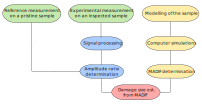
\includegraphics[width=1\linewidth]{Chapter_3/flowchart}
	%	\end{center}
	\caption{A flowchart representing the process for damage size estimation.}
	\label{fig:Flowchart}
\end{figure}
The \ac{madif} indicates the damage size according to measured damage index \(I\) normalized by the value obtained for the pristine sample \(I_{ref}\).
In the paper, two types of damage index \(I\) are considered: the energy \(I_{eng}\) and the maximum value of the half-width of the first package arrived in the sensor \(I_{amp}\), and these are defined as:
